
\documentclass[12pt]{beamer}
\mode<presentation>{\usetheme{Madrid}} % Either Madrid or Rochester

\usefonttheme{professionalfonts}
\usenavigationsymbolstemplate{}


\usepackage{graphicx}


\usepackage[utf8]{inputenc}
%\usepackage[T1]{fontenc}
\usepackage{palatino}
%\usepackage{euler}
%\usepackage{amsmath}
%\usepackage{amsthm}
%\usepackage{amssymb}
%\usepackage{amsthm,geometry}  
%\usepackage[colorlinks=true]{hyperref}

\newtheorem{cor}{Corollary}
\newtheorem{lem}{Lemma}
\newtheorem{thm}{Theorem}
\newtheorem{defin}{Definition}
\newtheorem{proposition}{Proposition}

%polices
\newcommand{\msf}{\mathsf}
\newcommand{\mrm}{\mathrm}
\newcommand{\mbf}{\mathbf}
\newcommand{\mbb}{\mathbb}
\newcommand{\mcal}{\mathcal}
%polices

\newcommand{\bra}[1]{\langle #1|}
\newcommand{\ket}[1]{|#1 \rangle}
\newcommand{\braket}[2]{\langle #1|#2\rangle}
\newcommand{\ketbra}[1]{\ket{#1}\bra{#1}}
\newcommand{\ketb}[2]{\ket{#1}\bra{#2}}
\newcommand{\ident}{\mathbb{I}}
\DeclareMathOperator{\tr}{\mathrm{Tr}}
\DeclareMathOperator{\rank}{rank}
\DeclareMathOperator{\polylog}{polylog}
\newcommand{\mdag}{^{\dag}} % dag operator
\newcommand{\demi}{\frac{1}{2}}

\newcommand{\state}{{\rho^{AE}}}
\newcommand{\mixed}{\frac{\mathbb{I}}{d_{A}} \otimes \rho^E}
\newcommand{\tra}{\tr_A}
\newcommand{\cypher}{\mathcal{E}}

\newcommand{\mpr}{{\mrm{Pr}}}
\newcommand{\mtr}[1]{\mathrm{Tr}\left(#1\right)}%trace
\newcommand{\mtra}[1]{\mathrm{Tr}_{A}\left(#1\right)}%trace
\newcommand{\mtrb}[1]{\mathrm{Tr}_{B}\left(#1\right)}%trace
\newcommand{\p}{^{\prime}}


%Nombres
\newcommand{\mbR}{\mathbb{R}}
\newcommand{\mbZ}{\mathbb{Z}}
\newcommand{\mbQ}{\mathbb{Q}}
\newcommand{\mbC}{\mathbb{C}}
\newcommand{\mbN}{\mathbb{N}}
\newcommand{\mbI}{\mathbb{I}}
\newcommand{\mE}[1]{\mcal{E}(#1)}
\newcommand{\mO}[1]{\mcal{O}(#1)}
\newcommand{\mbE}{\mathbb{E}}
%Nombres

%notation de circuit
\newcommand{\mh}{\mathrm{H}}
\newcommand{\mx}{\mathrm{X}}
\newcommand{\my}{\mathrm{Y}}
\newcommand{\mzz}{\mathrm{Z}}
\newcommand{\ms}{\mathrm{S}}
\newcommand{\mt}{\mathrm{T}}
\newcommand{\mamp}{\frac{1}{\sqrt{2}}}
\newcommand{\cnot}{\mathrm{CNOT}}
\newcommand{\msx}{\sigma_{x}}
\newcommand{\msy}{\sigma_{y}}
\newcommand{\msz}{\sigma_{z}}

%Des choses essentielles ˆ la beautŽ d'un papier
\setlength{\parindent}{0cm}
\setlength{\parskip}{2ex plus 0.5ex minus 0.5ex}

% Pour cette présentation
\newcommand{\aeq}{\approx_{(a)}}
\newcommand{\wtA}{\widetilde{A}}
\newcommand{\wtB}{\widetilde{B}}
\newcommand{\whA}{\widehat{A}}
\newcommand{\whB}{\widehat{B}}
\DeclareMathOperator{\Typ}{typ}

% ivan custom
\newcommand{\be}{\begin{equation}}
\newcommand{\ee}{\end{equation}}
\newcommand{\e}{  \ensuremath{\mathcal E} }
\newcommand{\x}{  \ensuremath{\mathcal X} }
\newcommand{\y}{  \ensuremath{\mathcal Y} }
%\def \mcX{\mathcal{X} } (better no?)
\newcommand{\m}{  \ensuremath{\mathcal M} }
\newcommand{\otimesc}{\negthickspace\otimes\negthickspace}	%close verison of \otimes 
\newcommand{\typ}{  \ensuremath{ T^{(n)}_\epsilon  } }
\newcommand{\jtyp}{  \ensuremath{ A^{(n)}_\epsilon  } }
%%% THEOREMS   %%%%%%%%%%%%%%
\theoremstyle{plain}
\newtheorem{Th}{Theorem}[section]
\newtheorem{Lem}[Th]{Lemma}
\newtheorem{Prop}[Th]{Proposition}
\newtheorem{Cor}[Th]{Corollary}
\theoremstyle{definition}
\newtheorem{Ex}[Th]{Example}
\newtheorem{Def}[Th]{Definition}
\newtheorem{Rem}[Th]{Remark}
\newtheorem{Quest}[Th]{Question}
\newtheorem{prf}{Proof}
%%% MATH SETS %%%%%%%%%%%%%%
\def \Tr{\textup{Tr}}
\def \c{\mathbb{C}}
\def \z{\mathbb{Z}}
\def \r{\mathbb{R}}
\def \n{\mathbb{N}}
\def \p{\mathbb{P}}
\def \q{\mathbb{Q}}

\title[Intro to QIT]{Introduction to quantum information theory}

\author[Ivan Savov]{Ivan Savov\\
McGill University\\
\strut\\
INTRIQ student conference}
\date{Jan 7, 2010}

\begin{document}

\begin{frame}
\titlepage
\end{frame}

%\begin{frame}
%	\frametitle{Outline}
%	\tableofcontent
%\end{frame}
%----------------------------------------------------------


\begin{frame}
	\frametitle{introduction}
	What is quantum information theory?

    \only<2>{
    = \\ \ \\
    \texttt{\structure{entropy}, \structure{channel}, let, theorem, log, bound, systems, probability, 
    proof, classical, quantum, \structure{information}, lemma, theory, ... }
    }

    \only<3->{
    More formally, QIT is the study of information processing tasks:
	\begin{itemize}
        \item Data compression
        \item Data transmission through a noisy channel
	\end{itemize}
    %quantum data and other quantum resources
    }
	%\emph{Quantum} information theory? Accomplishing these tasks with \emph{quantum} data or using quantum resources.
\end{frame}





%\begin{frame}

%\frametitle{Introduction}
%So what's in this thesis? A general method to solve quantum information theory problems based on removing correlations between quantum systems. More specifically:
%\begin{itemize}
%	\item A theorem that says how to remove correlations (``decouple'')
%        \item \cite{H98,SW97} .
%	\item How it can be used to recover many important QIT theorems
%	\item New coding theorems for quantum channels with side information at the transmitter and broadcast channels
%	\item A way to lock classical correlations in quantum states
%\end{itemize}
%\end{frame}

\begin{frame}
	\frametitle{outline}
	\begin{itemize}
		\item Classical information theory 
			\begin{itemize}
				\item Source coding = compression
				\item Channel coding
			\end{itemize}
		\pause  \item Quantum version
		\item \pause Three important results in QIT
		\item \pause What I do
		\item \pause Big picture
	\end{itemize}
\end{frame}





%\section{classical information theory}

%\subsection{Intro}

\frame{
		\frametitle{Shannon}
		\begin{columns}[c]
		\column{2in}
		\begin{itemize}
		\item C. Shannon in his 1948 paper titled \\ 
			``{\it A mathematical theory of communication}''
		 	\cite{S48} laid the foundations of what is known today as 
			Information Theory. \\ 
			\ \\
			\ \\
		\item He was the first to look at information sources as statistical objects.
		\end{itemize}
	
		\column{1.5in}
%		\framebox{ \begin{centering}	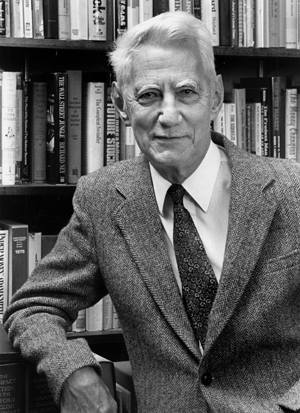
\includegraphics[width=1.5in]{Shannon} \end{centering} 			  }
				\framebox{ \begin{centering}	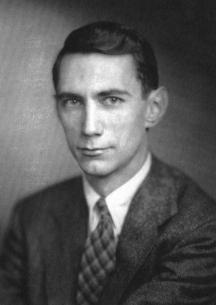
\includegraphics[width=1.5in]{Claude_Elwood_Shannon.jpg} \end{centering} 			  }
				
		\small{Claude Shannon (1916-2001) }
		\end{columns}
}
	

\frame{
	\frametitle{example 1: at the coffee shop}
	\begin{itemize}
	\item Let $X$ be the type of coffee you order
	\item It can only be one of two choices ``Mild'' or ``Dark''
	
	\item Suppose you are equally likely to pick both kinds:
		\begin{eqnarray*}
			\Pr\{X=\text{`M'}\} \ &=&\  0.5, \\
			\Pr\{X=\text{`D'}\} \ &=&\  0.5.
		\end{eqnarray*}
	\item Difficult to guess.
	\end{itemize}
}	
	
\frame{
	\frametitle{example 2: border control}
		\begin{itemize}
		\item 	Canadian border control point near Sutton
				 sends a status message $M$ to Ottawa 
		\item 	The possible messages are:
			\begin{itemize}
			\item	No one has attacked, which occurs 99.7\% of the time: \mbox{$\Pr\{M\!=\!`N'\}\!=0.997$}
			\item	The Americans have attacked: $\Pr\{M=`A'\}=0.002$
			\item	The Russians have attacked: $\Pr\{M=`R'\}=0.001$ 
			\end{itemize}
		\item In this scenario, one of the outcomes, $N$, is much more likely than all the others.
%		\item If we were to shut down the remote outpost and instead guess $M=\alpha^0$ every hour, we would only
%	be wrong 0.3\% of the time! Of course, implementing such an approximate border defense system 
%	is a silly idea, but in other situations an approximate result is just as good as the exact one.
		\item Easy to guess.
		\end{itemize}

}	
	

\frame{
	\frametitle{information theory = information statistics}
	\begin{itemize}
	\item 	In general, we will view an information source as 
			an \emph{alphabet} $\x$ which has an associated probability distribution $p(x)$.
			\ \\
			\ \\
	%\item 	This simple view of information sources allows us to do many useful things. \ \\
	\item	How do you quantify information ?
	
	\end{itemize}
}


%\subsection{Basics}

\frame{
	\frametitle{entropy}
	
	\begin{Def}[Shannon entropy] Given a statistical source over 
				the alphabet $\x$ with probability function $p(x)$, the quantity 
		\be
			H(X)= - \sum_{x_i \in \x}  p(x_i) \log p(x_i)
		\ee
		is the \emph{Shannon Entropy} of the source.
	\end{Def}
	\begin{itemize}
	\item 	The entropy of an unknown source measures our \emph{uncertainty} about it. \\
	\item 	The entropy of a known source measures how much \emph{information} we learn 
			on average from that source.		
	\end{itemize}
}


\frame[shring=20]{
		\frametitle{back to the examples}
		
		\begin{itemize}
		\item 	The information contained in your coffee order is:
				\be \nonumber
					H(X) = - 0.5\log0.5 - 0.5\log0.5 = -\log0.5 = \log2 = 1 \ [\textup{bit}].
				\ee
				In other words, you communicate one bit of information every time you order.
				
		\item 	The entropy of an outpost message is only:
				\be \nonumber
					\! \! \! \! \! \! \! \! \! \! \! \! \! \! H(M) = \! - 0.997\log0.997 - 0.002\log0.002 - 0.001\log0.001 \! \! = 0.032 \ [\textup{bits}].
				\ee
		\item 	Therefore, every coffee order carries about 30 times more information than a message from the 
				distant outpost.
		\end{itemize}
}
				
				
%	in other words, before we learn the value of $X$ we are maximally uncertain. Also, every time we learn the value 
%	we are gaining 1 bit of information.\\
%	On the other hand a binary source $Y$ with $Pr\{Y=0\}=0.1$ and $Pr\{Y=1\}=0.9$ only has an entropy of 0.47 bits.\\


%
%\frame{
%	\frametitle{multiple sources}
%	\begin{itemize}
%	\item Consider two sources $X$, $Y$ $\sim p(x,y)$, marginals: $p(x)$, $p(y)$.
%	\item The sources may or may not be correlated.
%	%\item New information theoretic quantities become relevant
%	\item 	Conditional entropy:  $ H(X|Y)		=	- \sum_{x,y} p(x,y) \log \frac{p(x,y)}{p(y)}$
%	\item 	Mutual Information:  $I(X:Y) = H(X)+H(Y)-H(X,Y)$
%	\item 	We can use a Venn-like diagram to represents the quantities: 
%			\begin{figure}[ht] 
%			\begin{center}
%				\input{FIGVENN.pic} 
%			\end{center}  
%			\end{figure}
%	\end{itemize}
%}




\frame{
	\frametitle{compression}
}



\frame{
	\frametitle{compression}

		\begin{columns}[c]
		\column{2in}
		\begin{itemize}
		\item Solved problem: \\ \ \\ \ \\
			\!\!\!\!\!\!\!\!\!	\texttt{gzip file.txt} 
		\end{itemize}
		\ \\ 
		\ \\ 
		\ \\


		\column{1.5in}
		\framebox{ \begin{centering}	
\includegraphics[width=1.5in]{winzip} \end{centering} 			  }
		
		\end{columns}
				\ \\
		\ \\
		\ \\
		\pause
		but that is not what we mean.... 

}

%\frame{
%	\frametitle{\textcolor{red}{theoretical} compression}
%	\begin{itemize}
%	\item Message is a sequence of 100 uses of source $X$.
%	\item Encode the message into a compressed string.
%	\item Compression rate:  
%		  \be
%		  	R	=	\frac{strlen(compressed)}{strlen(message)}
%		  \ee
%	\item 	Coding theorem: [Shannon 1948]\\
%			\textit{If compression rate $R>H(X)$, then there exists a 
%					 compression scheme that works.}
%		  \ \\
%		  \ \\
%	\item How? \\
%		  \ \ \ typical sets, typical sequences
%	\end{itemize}
%}


%\subsection{Compression}
\frame{
	\frametitle{compression (a.k.a source coding)}
	% Without going into too much detail, it is possible to get an intuitive understand of 
	% the Shannon source coding theorem.
	\begin{Def}[compression protocol]
		If $X_1,X_2,\ldots X_n$ are iid $\sim p(x)$ for $x\in \mathcal{X}$ then compression to 
		rate $R$ is possible if there exits:
		\begin{eqnarray}
			E_n:\x^n	 	& \rightarrow & 	\m \qquad |\m| = 2^{nR} \\
			D_n:\m 			& \rightarrow &		\x^n 
		\end{eqnarray}
		and $Pr\{X^n \neq Y^n\} \xrightarrow{n \to \infty} 0$ where $Y^n = \left(D_n\circ E_n\right)X^n$.
	\end{Def}
	\begin{Th}[Shannon bound on compression]
	Compression is possible for any $R>H(p)$.
	\end{Th}	
	How? --- typical sets, typical sequences
	
}



%\subsection{Channel Capacities} 											
\frame{
	\frametitle{channel coding}
}


%\subsection{Channel Capacities} 											
\frame{
	\frametitle{communication channels}
	\begin{itemize}
		\item Consider some communication medium like an optical, electrical or radio link 
		\item The sender (Alice) wants to communicate with the receiver (Bob) 
		\item The channel is \textcolor{red}{noisy}
		\item	You input symbol $x$ and out comes symbol $y$ according to some $p(y|x)$
		\begin{displaymath}
			\fbox{Sender A } \xrightarrow{\ \ X\ \ } \fbox{ Channel $p(y|x)$ }  \xrightarrow{\ \ Y\ \ } \fbox{Receiver B}
		\end{displaymath}
		%\item How mucThe channel capacity is the maximum number of bits of information that B can receive reliably.
	\end{itemize}  
}


\frame{
	\frametitle{channel coding}
	\begin{itemize}
	\item Alice's message $m$ is one of $N$ possible messages
	\item Alice encodes the message into an $n$-bit codeword $X^n$.
	\begin{displaymath}
		m \rightarrow \fbox{Encoding} \rightarrow X^n \xrightarrow{\ \ \  \text{Channel } p(y|x) \ \ }  Y^n \rightarrow \fbox{Decoding} \rightarrow \tilde{m}
	\end{displaymath}
	\item Upon reception, Bob will try to guess $m$ by decoding the received symbols $Y^n$.
	%\item The \emph{channel capacity} is the largest $R$ such that this can be done without errors
	\end{itemize}
}



\begin{frame}
\frametitle{channel coding}
This is the picture:
    \begin{figure}
    \hspace{-2.3cm}\scalebox{0.8}{\input{canal-iid-enc-dec.pdf_t}}
    \end{figure}
The \emph{rate} of this code is the ratio $R= (\log N)/ n$.  % $\Pr\{ m \neq \hat{m} \} \rightarrow 0$.
\end{frame}


\frame{
	\frametitle{channel capacity formula}
	\begin{Th}[channel capacity] 
		The information channel capacity of a discrete memoryless channel is
		\be
			C = \max_{p(x)} I(X:Y)
		\ee
	where the maximum is taken over all possible input distributions $p(x)$.  \cite{S48}.
	\end{Th}
	\begin{itemize}
		\item There exist codes of rates arbitrarily close to $C$ that have negligible probability of error.
		\item Any attempt to send at a rate $R>C$ will result in large errors.
	\end{itemize}
}



%
%
%\frame{
%	\frametitle{The Encoding}
%	The idea behind the such a compression protocol is:
%	\begin{itemize}
%	\item Reject any sequence that is not typical. \\
%		  The AEP guarantees us that we will be seeing very few of those  $\rightarrow$ very few mistakes. 
%	\item Label the typical sequences with a string of length nR.
%	\item We know that
%	\be
%		\lvert \typ \rvert \leq 2^{n[H(X)+\epsilon]} 
%	\ee
%	and thus for any $R > H(X)$ we will be able to index all the typical sequences with strings of $nR$ bits.
%	\end{itemize}
%}




	









\frame{
	\frametitle{quantum mechanics}
}

\frame{
	\frametitle{computer science view}

	\begin{itemize}
	\item change bits \\
			$x = 0 \ or\ 1$ \ \ 	(two level systems) \\
	 	to qubits \\
			$\ket{x} = \alpha\ket{0} +\beta\ket{1}$  \ \ (vectors in $\c^2$) \\
		and mixed states $\rho, \sigma$ 
	\item	idealized system with only 2 quantum states
	\item change logic gates to quantum gates (Unitary operators) 
	\ \\
	\end{itemize}
}




%\section{quantum information theory}
%\subsection{Change of context}


\frame{
	\frametitle{quantum information theory}
	\begin{itemize}
	\item Very similar to classical information theory
	\item Replace Shannon entropy with von Neumann entropy
			\begin{Def}[von Neumann Entropy] A quantum system described by the density matrix $\rho$ has von Neumann 
			entropy $S(\rho)$ given by the expression:
			\be
				S(\rho) = - \Tr(\rho \log\rho)
			\ee
			\end{Def}
	\ \\
	\ \\
	\item Same story all over again: mutual information, quantum channel capacities, quantum compression, etc.
	\end{itemize}
}	
%
%\frame{
%	\frametitle{something new: entanglement}
%	\begin{itemize}
%	\item new quantum resource
%	\item quantum correlation
%	\ \\
%	\ \\
%	\item  (no time for details)
%	\end{itemize}
%}


%
%\frame{
%	\frametitle{Definition}
%	\begin{Def}[von Neumann Entropy] A quantum system described by the density matrix $\rho$ has von Neumann 
%	entropy $S(\rho)$ given by the expression:
%	\be
%		S(\rho) = - \Tr(\rho \log\rho)
%	\ee
%	\end{Def}

%}	


\frame{
	\frametitle{new quantum resources}
	\begin{itemize}
		\item	Quantum Bit (q-bit) 
		\item	Shared maximally entangled pairs:  [q\,q] (e-bits)\\
					ex: $\frac{1}{\sqrt{2}}(\ket{00}+\ket{11})$
		\item e-bits have no analog in classical information theory 
		\item	Coherent Bits: $[q \to qq]$ (co-bits)
		\item	Noiseless Quantum Channel: $[q \to q]$
		\item	Noisy channel: $\{ q \to q \}$ usually denoted $\mcal{N}$. 
	\end{itemize}
	}	




				
%%%%%%%%%%%%
%%%%%%%%%%%% SURVERY OF RESULTS IN QUANTUM INFORMATION 
%%%%%%%%%%%%		

\frame{
	\frametitle{quantum information theory}
	\begin{itemize}
		\item Can you do cool tricks with EPR pairs? \\
		$\ket{\Psi} = \frac{1}{\sqrt{2}}(\ket{00}+\ket{11})$ \\
		\ \\
		\item Can we compress quantum information? \\
		\ \\
		\item	Can you send information through a quantum channel?  \\
		\ \\
		\ \\
		\pause \item YES to all of the above 
	\end{itemize}
	}	




		

\frame{
		\frametitle{2$\times$ brilliant trivialities}
		\begin{itemize}
			\item 	Superdense Coding [Bennett, Wiesner 1992]:\\
					\be
						[q\,q]+[q \to q] 	\geq	2[c \to c]
					\ee
					
			\vspace{0.2cm}
			\item 	Teleportation [BBCJPW 1993]:\\
					\be
						[q\,q]+2[c \to c] \geq	[q \to q]
					\ee
					
		\end{itemize}
		}



\frame{
	\frametitle{who is this?}
	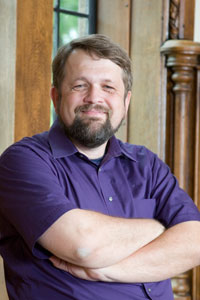
\includegraphics[width=2in]{quantum_people/SchumacherBE.jpg}

}

	
\frame{
	\frametitle{Schumacher compression}
	\begin{itemize}
	\item Start with $\rho^{\otimes n}$ ($n$ copies of state $\rho$).
	\item How much can you compress? \\
	\ \\
%	\item Compression rate:  
%		  \be
%		  	Q	=	\frac{strlen(compressed)}{strlen(message)}
%		  \ee
	\begin{Th}[quantum source coding]
		An i.i.d. quantum source $\rho$ can be compressed at
		a rate $R$ if $R > S(\rho)$ and cannot if $R < S(\rho)$.	\ \ \ [Schumacher 1995]
	\end{Th}
	
	\ \\
	\item How? \\
		  \ \ \ typical subspaces
	\end{itemize}
}



	
\frame{
	\frametitle{quantum data compression}
	\includegraphics[width=4.8in]{mark_diagrams/SchumacherDiagram.png}
	
}

% channel capactity




\frame{
	\frametitle{who are these people?}
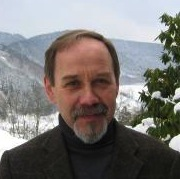
\includegraphics[height=1.6in]{quantum_people/Holevo,_Alexander2.jpg}
\ \ \ 
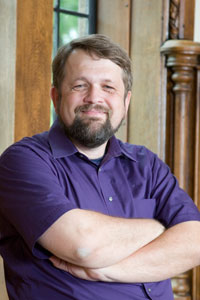
\includegraphics[height=1.6in]{quantum_people/SchumacherBE.jpg}
\ \ \ 
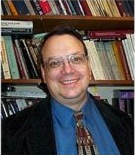
\includegraphics[height=1.6in]{quantum_people/mike_westmoreland.jpg}

}





%%
%\begin{frame}
%	\frametitle{Entanglement assisted}
%	\begin{itemize}
%		\item $EAC = max_\rho I(A;B) $
%		\item $EAQ = max_\rho \frac{1}{2} I(A;B) $
%	\end{itemize}
%\end{frame}


\begin{frame}
	\frametitle{classical capacity of quantum channel}
    
    Holevo, Schumacher and Westmoreland found a formula
    for the classical capacity of a quantum channel [H98,SW97].

	\begin{Th}
		The classical capacity of a quantum channel $\mcal{N}$ is
		given by
		\be
	       		C(\mcal{N}) = \max_\rho I(A;B) 
	    	\ee
		where $\rho$ is the output state 
		    \be
		        \rho = \sum_x p(x) \ketbra{x}_A \otimes \mcal{N}\!({\sigma_x})_B.
		    \ee
		    and $\sigma_x$ are the input symbols.
	    \end{Th}
		
		%\begin{itemize}
		%	\item .
		%	\item .
		%\end{itemize}
\end{frame}




\frame{
	\frametitle{who are these people?}
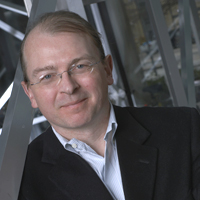
\includegraphics[height=1.6in]{quantum_people/Lloyd_Seth.jpg}
\ \  \ \
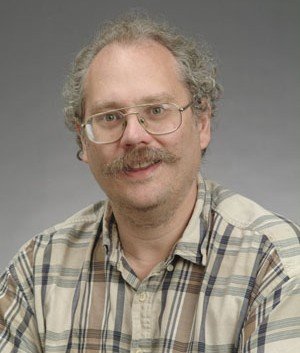
\includegraphics[height=1.6in]{quantum_people/shor-peter.jpg}
\ \  \ \ 
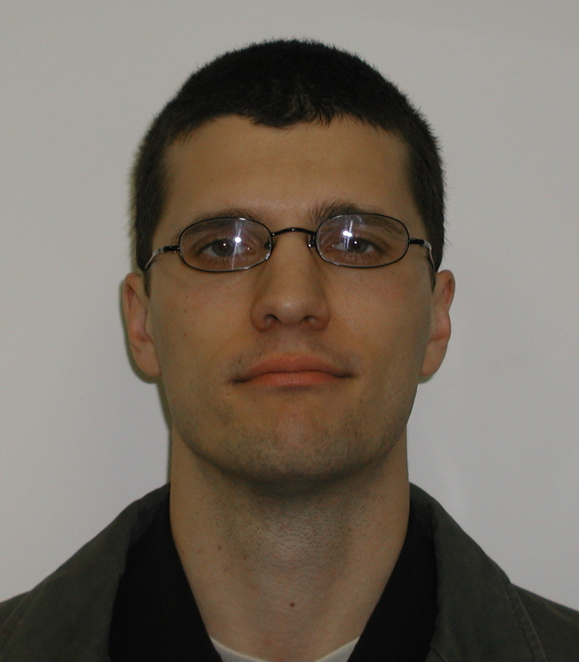
\includegraphics[height=1.6in]{quantum_people/devetak.jpg}

}



\begin{frame}
	\frametitle{quantum capacity}
    Lloyd, Shor and Devetak independently proved a formula for the quantum capacity
    of a channels.
    
    \begin{Th}[LSD Theorem]
    
    Consider the input state $\rho^{AA'}$, half of which is sent
    through the channel $\mcal{N}$ to obtain $w^{AB} = \mcal{N}^{A'\to B}(\rho^{AA'})$.
    Define the quantity 
    \be
        Q^{(1)}(\mcal{N}) = \max_\rho  (S(B)_w - S(AB)_w).
    \ee
    The quantum capacity $Q$ of the channel $\mcal{N}$ is given by the regularization 
    of the $Q^{(1)}$ quantity
    \be
        Q(\mcal{N}) = \lim_{n\to \infty} \frac{Q^{(1)}(\mcal{N}^{\otimes n} )}{n}.
    \ee 
    [L97, S00, D03]
    \end{Th}
    
	\begin{itemize}
		\item .
		\item picture with channel being used in blocks of 2.
	\end{itemize}
\end{frame}




\frame{
	\frametitle{next time...}
	
	Next time someone asks you what kind of research you do,  \\
	\ \\
	\pause 
	say you are working on the LSD Theorem.
	\ \\
}


\frame{
	\frametitle{what do i do?}
	\ \\
	\ \\
	\pause multiparty stuff 
}

	
\frame{
	\frametitle{distributed compression}

	
	Initial  state: $\ket{\psi}^{A_1A_2\cdots\!A_mR}$
			
%		\begin{itemize}
%			\item Graphically represented:
%		\end{itemize}		
		\begin{figure}[ht] \begin{center}
	        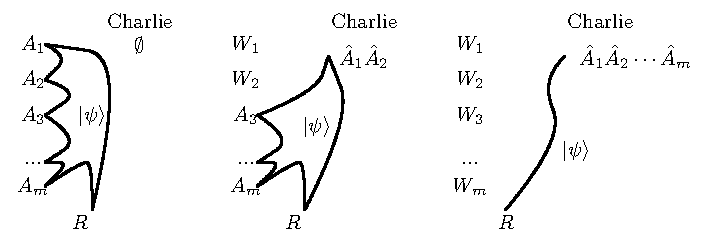
\includegraphics[scale=0.9]{figures/newmpFQSW.pdf}
	        \caption{ Quantum correlations at three different stages of the protocol. }
%	            Originally the state $\ket{\psi}$ is shared between $A_1A_2\cdots A_m$ and $R$.
%	            The middle picture shows the protocol in progress.
%	            Finally, all systems are received by Charlie and $\ket{\psi}$ is now shared between
%	            Charlie's systems $\widehat{A}_1\widehat{A}_2 \cdots \widehat{A}_m$ and $R$.            }
	        \label{fig:mpFQSWdiagram}
	    \end{center}
	    \end{figure}
	    \vspace{-1cm}
	    Final state:  $\ket{\psi'}^{CR} \approx \ket{\psi}^{A_1A_2\cdots\!A_mR}$.  [Avis, Hayden, Savov 07]
}


%\frame{
%	\frametitle{multiparty squashed entanglement}
%	
%	bah...

%}






%\frame{
%	\frametitle{the rate region}
%	\begin{itemize}
%	\item If rate tuple $(Q_1,Q_2,Q_3)$ is possible, then it is inside the rate region
%	\item i.e. there exists a distributed compression protocol that can achieve these rates
%			\ \\
%			\ \\
%			\ \\
%	\item Rate region is a polyhedron
%	\item Nice regular shape: supermodular polyhedron
%	\end{itemize}
%}

%

\frame{
	\frametitle{entanglement assisted QECC}
	\begin{itemize}
	\item quantum error correcting codes (QECC) are important for all applications 
	\item what if sender and receiver share EPR pairs? \\
		can build more interesting QECC codes  [Brun, Devetak, Hsieh 06]
	\item what if state is split between two senders? \\
		 by using entanglement can use regular QECC codes [Brun, Wilde]
	\item what if more than two senders? \\
		work in progress.... 
	\item nice because we get explicit code construction 
	
	\end{itemize}
}

%
%\frame{
%	\frametitle{my thesis}
%	Abstract:
%	\begin{quotation}
%	We partially solve the multiparty distributed
%	compression problem where multiple parties use quantum communication
%	to faithfully transfer their shares of a state to a common receiver.
%	We build a protocol for multiparty distributed compression based on the fully
%	quantum Slepian-Wolf protocol and prove both inner and outer bounds on the
%	achievable rate region. 
%	\end{quotation}
%}

%

%











\begin{frame}
	\frametitle{resum\'e}
	\begin{itemize}
        \item Information theory can be generalized to analyze quantum information
       % \item Yields a rich theory, surprising conceptual simplicity
       \item Another way to think about quantum mechanics: \\
                information, correlations, decoupling , compression, transmission
        \item Very young field
        \item Lots of open problems
        \item Needs people from different backgrounds
	\end{itemize}
\end{frame}

%
%\begin{frame}
%	\frametitle{What about the future?}
%	\begin{itemize}
%	\item We have not used the decoupling theorem to its full potential yet
%	\item Could be used to show protocols for channels with memory
%	\item Other types of channels
%	\item Optimality?
%	\item Explicit protocols (with high concentration)
%	\end{itemize}
%\end{frame}


\begin{frame}
	\frametitle{quantum information science}
	\begin{itemize}
	\item many branches dealing with specific aspects
        \item quantum crypto = \texttt{alice bob protocol key information quantum communication bit teleportation channel eve bits ...}
        \item non-locality = \texttt{ bell quantum local inequality correlations EPR ... }
        \item error correcting codes = \texttt{ qubit quantum gates error code computation operations ...}

        \item quantum algorithms = \texttt{ quantum algorithm computation computer complexity probability problem number search classical ... }
	\end{itemize}
\end{frame}




\begin{frame}
	\frametitle{the end}
	\begin{center}
		\huge thanks for your attention!
	\end{center}
\end{frame}

\begin{frame}[allowframebreaks]{References}
    \bibliographystyle{alpha}
    \bibliography{thesis}
\end{frame}


\end{document}
